\documentclass[11pt,a4paper]{article}

\usepackage[margin=.75in]{geometry}
\usepackage{amsfonts}
\usepackage{amsmath} % \text{}
\usepackage{amssymb}
\usepackage{amsthm}
\usepackage{fancyvrb}
\usepackage{graphicx}

% sans font
\renewcommand*{\familydefault}{\sfdefault}
\renewcommand*\sfdefault{phv}

% indentation and paragraph spacing
\setlength{\parindent}{0em}
\setlength{\parskip}{.5em}

%\usepackage{color}
\usepackage{xcolor}
\definecolor{red}{RGB}{154,00,00}
\definecolor{pink}{RGB}{255,20,147}
\definecolor{lightgray}{rgb}{0.97,0.97,0.97}

\usepackage{hyperref}
\hypersetup{
	colorlinks,
	linkcolor=red,
	citecolor=red,
	urlcolor=red
}

% for listing code
\usepackage{listings}

\lstdefinestyle{lststyle}{
	backgroundcolor=\color{lightgray},
	commentstyle=\color{blue},
	keywordstyle=\color{red},
	numberstyle=\tiny\color{black},
	stringstyle=\color{pink},
	basicstyle=\small\ttfamily,
	breakatwhitespace=false,
	breaklines=true,
	captionpos=t,
	keepspaces=true,
	numbers=left,                    
	numbersep=5pt,                  
	showspaces=false,                
	showstringspaces=false,
	showtabs=false,                  
	tabsize=3,
	stepnumber=1,
	frame=tb,
	escapeinside={($}{$)}
}

\lstset{style=lststyle}

\begin{document}

\section*{Automated Report}

This report was automatically generated by executing \verb|./automate|. The executable \verb|automate| was created by compiling \verb|automate.f95| using the \verb|gfortran| compiler:
\begin{Verbatim}[frame=single]
gfortran automate.f95 -o automate
\end{Verbatim}
To create Table~\ref{tab:automate}, \verb|automate| outputs the \verb|.tex| file \verb|table.tex| that is input to this document. To plot the graphs $y=\sin x$ and $y=\cos x$, \verb|automate| outputs the data file \verb|figure.dat| and calls the gnuplot script \verb|automate.plt| that plots the data. 

Table~\ref{tab:automate} lists values of $\sin x$ and $\cos x$ at $\displaystyle x=i\frac{\pi}{5}$ for $i=0,1,2,\ldots,10$.
\begin{table}[h!]
\centering
 \begin{tabular}{|c|c|c|} \hline
 $x$ & $\sin x$ & $\cos x$ \\ \hline
   0.00000000     &   0.00000000     &   1.00000000     \\
  0.628318548     &  0.587785244     &  0.809017003     \\
   1.25663710     &  0.951056540     &  0.309016973     \\
   1.88495576     &  0.951056480     & -0.309017152     \\
   2.51327419     &  0.587785184     & -0.809017062     \\
   3.14159274     &  -8.74227766E-08 &  -1.00000000     \\
   3.76991153     & -0.587785542     & -0.809016764     \\
   4.39822960     & -0.951056480     & -0.309017092     \\
   5.02654839     & -0.951056480     &  0.309017122     \\
   5.65486670     & -0.587785304     &  0.809016943     \\
   6.28318548     &   1.74845553E-07 &   1.00000000     \\
 \hline \end{tabular}

\caption{Values of $\sin x$ and $\cos x$.}
\label{tab:automate}
\end{table}

Figure~\ref{fig:automate} plots the values of $\sin x$ and $\cos x$ at $\displaystyle x=i\frac{\pi}{5}$ for $i=0,1,2,\ldots,10$.
\begin{figure}[h!]
\centerline{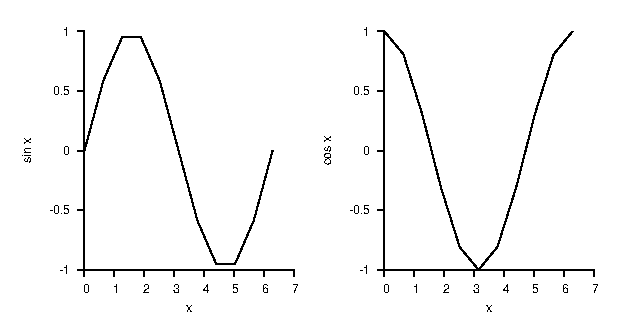
\includegraphics[width=.5\textwidth,keepaspectratio]{figure.eps}}
\caption{Plots of $y=\sin x$ and $y=\cos x$.}
\label{fig:automate}
\end{figure}

The source code for \verb|automate.f95| is listed as follows.

\hrulefill\verb| automate.f95 |\hrulefill\vspace{-2mm}
\lstinputlisting[language=fortran,frame=bottomline]{automate.f95}

\end{document}
